\documentclass[11pt]{article}
\usepackage{graphicx}
\usepackage{cite}
\usepackage{xcolor}
\usepackage{listings}

\def\UrlBreaks{\do\/\do-}
\lstset{language=Fortran, 
  basicstyle=\small\ttfamily, 
  %identifierstyle=\color{green}, 
  numbers=left,
  commentstyle=\color{red}, 
  keywordstyle=\color{blue}, 
  showstringspaces=false 
}


\author{S.~V.~Adams, S.~Cusworth, C.~M.~Maynard, S.~Mullerworth and others}
\title{Report on LFRic computational performance 2019}
\date{\today}


\begin{document}
\maketitle
\medskip
\section{Introduction\label{sec:intro}}
The LFRic infrastructure is designed to host a dynamical core (Gung Ho)
that is scalable to a very large degree across a distributed memory
computer. This is typically expressed over MPI. LFRic is also designed
to accommodate different programming models to target different
processor architectures. Currently, OpenMP 2.0 is supported for shared
memory parallelism on CPUs. This is being extended to support OpenACC
to target both shared memory parallelism and Instruction Level
Parallelism (IPL) on GPUs. Moreover, the infrastructure has been
extended to support parallel, asynchronous I/O using the XIOS
client/server framework.
Other developments include the abstract solver API which allows for great
flexibility in constructing different solvers, redundant computation
algorithms into halo regions which boost the efficiency of shared
memory and reduce the amount of communication and finally a Multigrid
solver which will enable a large reduction in the cost of global communication.
Much of the model infrastructure is described in~\cite{LFRic}.

The LFRic model uses PSyclone to generate the Parallel System or PSy
layer. Here, data parallelism across the horizontal mesh is used,
exploiting both distributed and shared memory parallelism. This
exploits domain specific information, known to the science developer
and encoded as Metadata in the kernel layer. However, to
fully exploit the ILP on more parallel architectures such as GPUs, it
is necessary to extend PSyclone to fully parse individual Fortran
statements in the Kernel layer and then, for example, annotate the
source code with directives such as OpenACC or OpenMP. This work is just beginning,
however, the micro-benchmark~\cite{lfric-microbenchmarks} suite has been
developed so compute intensive kernels can be used to explore what kernel
optimisation can be developed which can then be generated by PSyclone in the full
model. The PSyclone Kernel Extractor (PSKE) is being developed to
allow the automated extraction of kernels, or more specifically a
driver with a dump file containing the necessary data for the looping
over the horizontal mesh and degrees of freedom without any of the
LFRic infrastructure.

LFRic uses Fortran 2003 Object Orientation programming to support many of the
features described above. This is a very powerful programming
style which aids software development by allowing a clear separation
of concerns between different areas of the code, promoting code re-use
and code development by disentangling dependencies. However, the lack
of compiler support, or more precisely, the proliferation of compiler
bugs which prevent the use of particular compilers, either without specific
code work arounds or even at all, is major problem. Development has
been severely delayed whilst compiler bugs have been isolated and
reported and work-arounds sought. The lack of working Fortran 2003
compilers remains a source of concern and must be considered a risk to
the project.

The strategy to obtain compute performance for LFRic has four main
strands. I/O performance is achieved by using the XIOS capability for
asynchronous parallel I/O in order to hide the cost of writing data.
Compute performance is achieved by enabling scalability, allowing
many agents to do computation. This comes at the cost of communication.
Local communication in the form of halo
exchange is reduced by employing a communication avoiding/reducing
algorithm of redundant computation into the halos and exploiting shared
memory threaded parallelism. Global communications are primarily in
the form of global sums required for iterative solvers. The global sum
is already vendor optimised both in the vendor supplied MPI library
implementation and the high-bandwidth, low-latency network of the
machine itself. The only way to reduce this cost and ultimate limit on
scalability is to use an algorithm with fewer global sums. This is the
Geometric multigrid pre-conditioner to the Helmholtz solver. The {\em
  on-node} compute performance of the LFRic code itself is examined by
considering the performance of computationally intensive kernels on
different processor architectures. The LFRic Microbenchmark suite can
be used to develop architecture specific optimisations.
The report is organised into sections on each of these four strands,
{\em viz.} I/O, local communication, global communication and
architecture specific optimisations.

\section{\label{sec:scale}Scaling Analysis}
The Gung Ho dynamical core uses an unstructured mesh to avoid a
singular pole which ultimately inhibits the scaling of the
UM. Examining the scaling behaviour of the model to see if it
performs sufficiently well is therefore important. To test the scaling a series
of model runs was performed. The version of the LFRic repository trunk
was $17483$. The code were compiled on the XCS with the Intel 17
compiler, at production level which is \verb+-O3+. The baroclinic wave
test was run on a $C576$ mesh. This roughly corresponds to a $17$km
horizontal resolution. The model was run with a $30$km lid and with
$30$ levels.  The time-step used was $180$s
seconds and the benchmarks were run for $100$ time-steps. The code was
profiled using the CrayPAT tool in sampling mode. 

\begin{figure}
\centering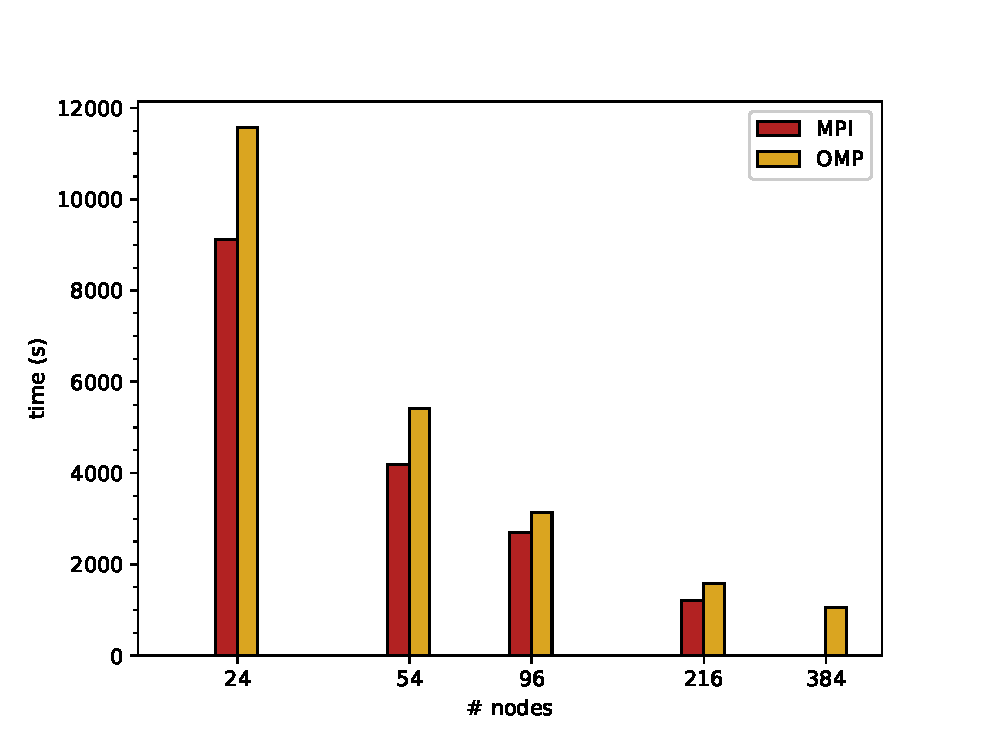
\includegraphics[width=1.0\linewidth]{figs/wc-scale.eps}
\caption{\label{fig:wc_scale}Wall-clock time strong scaling of the 
  Baroclinic wave test. In red, labelled MPI is an MPI only
  version. In yellow, labelled OMP is the hybrid MPI+OpenMP version.}
\end{figure} 

Shown in figure~\ref{fig:wc_scale} is the strong scaling of the whole
model up to $384$ nodes. The MPI only version ran with $36$ MPI ranks
per node. The hybrid version ran with $6$ MPI ranks per node and $6$
openMP threads per MPI rank. The MPI only version on $384$ nodes
crashed during the partitioning phase with an Out Of Memory (OOM)
error. The global mesh is read in by every MPI rank and then
partitioned. This can cause memory problems for large meshes on larger
node counts. This can be solved by a single rank per node reading in
the mesh and broadcasting the partition. The $24$ node hybrid job ran
out of time after 3 hours at $93$ time-steps, so the run time has been
estimated from the log data. This data is also shown in
table~\ref{tab:scale-data}.

\begin{table}
\centering
\caption{\label{tab:scale-data}Wall-clock time of execution of the whole code (WC), User
  code (U), Halo Exchange (HE) and Global Sum (GS) in seconds. Also
  shown is the Local Volume per MPI ranks (LV) and the Halo Size (HS)
  measured in number of horizontal cells.}
\begin{tabular}{r|rrrr|cr}
N & WC & U & HE & GS & LV & HS  \\
    & \multicolumn{4}{c|}{time (s)} & \multicolumn{2}{c}{cells} \\ \hline\hline
     &  \multicolumn{4}{c|}{MPI}& \\
$24$  & $9126$ & $4107$ & $788$ & $502$ & $48\times 48$ & $196$ \\
$54$  & $4196$ & $3139$ & $411$ & $470$ & $32\times 32$ & $132$ \\ 
$96$  & $2693$ & $1508$ & $380$ & $679$ & $24\times 32$ & $100$ \\ 
$216$ & $1202$ & $566$  & $302$ & $174$ & $16\times 16$ & $68$  \\ 
$384$ & $--$   & $--$   & $--$  & $--$  & $12\times 12$ & $54$ \\\hline
  & \multicolumn{4}{c|}{Hybrid} & \\
$24$ &$11566$ & $--$    & $--$  & $--$ & $96\times 144$ & $484$ \\
$54$ & $5410$  & $2732$ & $1282$ & $887$ & $64\times 96$ & $324$ \\
$96$ &$3140$  & $1332$ & $895$ & $562$ & $48\times 72$ & $244$ \\
$216$ &$1585$  & $468$ & $485$ & $384$ & $32\times 48$ & $164$ \\
$384$ &$1059$  & $222$ & $310$ & $322$ & $24\times 32$ & $124$ \\\hline
\end{tabular}
\end{table}

The model shows good scaling for both the MPI and hybrid programming
models. The parallel efficiency is reasonable, the $216$ node job uses
$9\times $ the resources of the $24$ node job and both the MPI and
hybrid version run more than $7\times $ faster. The hybrid code for the
$384$ node job which has $16\times $ the resource of the $24$ node
job, runs approximately $11 \times$ faster.

Compared to the scaling runs performed with the {\em Fallow Deer} (FD)
release of LFRic and reported in~\cite{LFRic} there is an apparent
change in the OpenMP behaviour. The FD scaling shows the hybrid version of
the code is faster than the MPI version, whereas the opposite is now
true for the data displayed here. It is unclear why this might be
so. The science problem and parallel code are broadly the same. The
major change is to the solver algorithm which uses the new solver
API. However, it is far from obvious why this would change the
behaviour.

The jobs have been profiled with CrayPAT and the data is shown in
table~\ref{tab:scale-data}. CrayPAT groups the data according certain
categories. User code (labelled ``U'') in the table and is the LFRic
code, in this case kernels such as the various matrix-vector
routines. The Halo Exchanges (labelled ``HE'') appear in the {\em ETC}
category as YAXT is compiled as a library, in this case without the
CrayPAT profiling, so it is unable to see that this ultimately calls
MPI. The Global Sums (labelled ``GS'') appear under {\em MPI} as the
global summation calls are in the LFRic infrastructure code.

The strong scaling of the user code is shown in
figure~\ref{fig:U_scale}\footnote{There is no hybrid data for 24 nodes
  as the model didn't run to completion so no profile was generated.}.
Both the MPI only and hybrid code show excellent scaling - the
communication costs are represented in other categories. For MPI
only, comparing the $24$ node to the $216$ node jobs, the User code
runs nearly $9\times$ faster for $9$ times the resource. The hybrid
version fares even better, showing super-linear scaling. Comparing the
$54$ node job to the $384$ node job, the user code runs more than
$12\times$ faster for $7.11\times$ the resource. This may well be due
to caching effects, once the local volume becomes small enough to fit
into cache.


\begin{figure}
\centering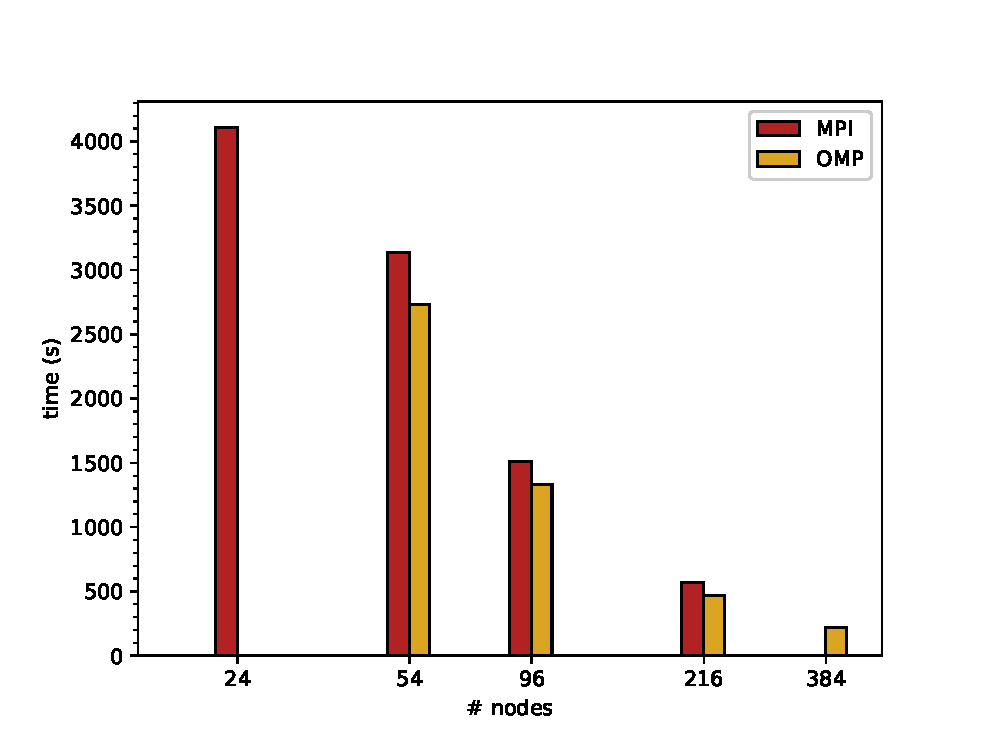
\includegraphics[width=1.0\linewidth]{figs/U-scale.eps}
\caption{\label{fig:U_scale}Wall-clock time strong scaling of the 
  User code from Baroclinic wave test.}
\end{figure} 

Shown in figure~\ref{fig:comms_scale} and Table~\ref{tab:scale-data}
is the strong scaling of the communication components as measured by
the CrayPAT tool. The halo exchanges for hybrid version of the code
takes significantly longer than the MPI only version. The time
difference accounts for the hybrid version being slower than MPI only.
The count of the number of halo exchanges (performed internally by
LFRic) is almost the same for the MPI and hybrid versions. The
difference is a few hundred out of a total of $1.3$ million. The are
not exactly the same because the global sum is not reproducible across
different partitions, so the evolution is slightly different. However,
after $100$ time-steps and many thousands of solver iterations, the
conservative fields are still the same to many orders of magnitude.

\begin{figure}
\centering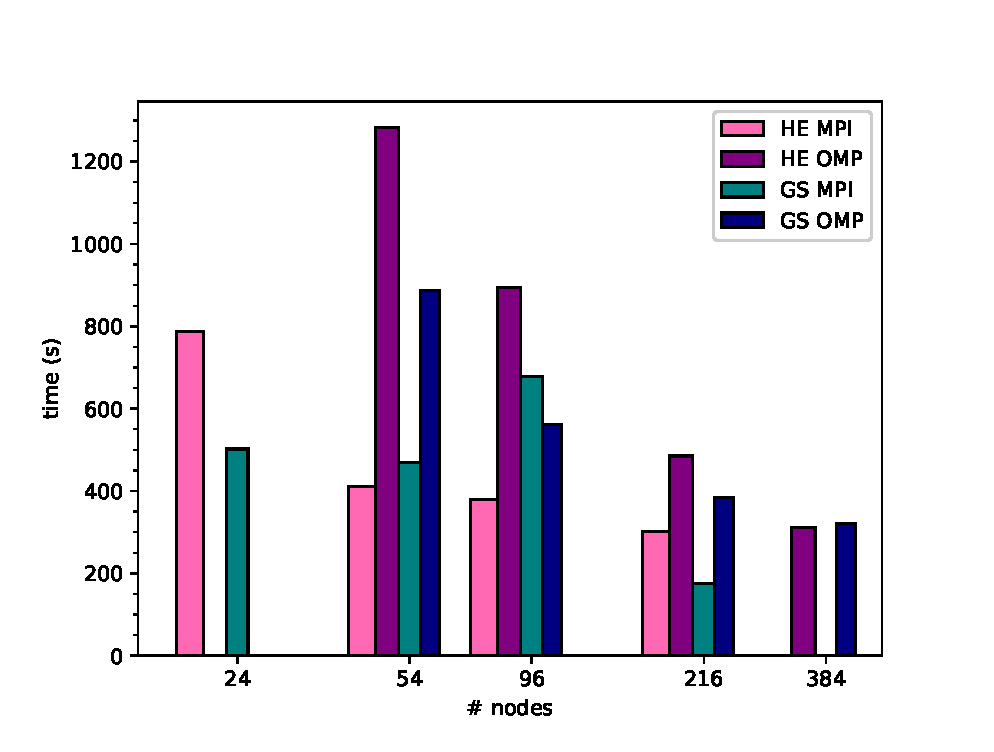
\includegraphics[width=1.0\linewidth]{figs/comms-scale.eps}
\caption{\label{fig:comms_scale}Wall-clock time strong scaling of the 
  communications costs of the Baroclinic wave test. HE denotes Halo
  Exchange and GS the Global Sum.}
\end{figure} 

The size of the halos is shown in Table~\ref{tab:scale-data}. The 
halos for the hybrid version are bigger than the MPI only version, as 
there are less MPI ranks, but there are less messages to send. As the 
hybrid version is running with six threads, it has six times less the 
number of messages. The hybrid version has fewer, but bigger MPI 
messages and moreover, will have less total data to send. It is not 
obvious why it should be so much slower. 

The global sums don't show a clear trend in the case of MPI only and
they appear to get faster with more nodes for the hybrid version. This
is perhaps counter intuitive as the global sum is latency bound and
should increase with the number of nodes. However, the aries network
employs adaptive routing so that the path taken for communication
depends on what other network traffic is occurring at the same
time. This results in the best use of the total network, but for an
individual application the communication cost may not be optimal and
worse, not deterministic.

To try and remove the effect of this variability, a Cray environment
variable \verb+GNI_BLAS+ was set to $2$ and the $96$ node jobs re-run.
Whist there was a difference between the run-times, the less adaptive
version was not consistently faster, nor did it change the balance
significantly. It should be noted that the communication cost
node imbalance for the hybrid mode is significantly higher than for MPI
only. The imbalance (defined as the variation across MPI ranks) is
around $15\%$ of the halo exchange cost, which rises to $30\%$ of a
much larger number for the hybrid version. For the global sum, again
there is a much larger variation for the hybrid version even if the total time spent in
global sums is reduced compared to MPI only. Changing the Cray
environment variable settings does not materially change this view. 

It is also not obvious why the hybrid version should now be slower
than MPI when the opposite was true in the fallow deer. In this data
the time-step is longer at $180$s and moreover, the fallow deer data
was not profiled using CrayPAT, but the time for $50$ time-steps
calculated from the logs. Shown in table~\ref{fig:fd_comp} is a
comparison of trunk at r17483 and the fallow deer release (labelled
FD). Clearly the hybrid version is now much slower. The trunk versions
uses the new solver API, so the solver is a different algorithm but it
is not doing a significantly different number of halo
exchanges. Neither the YAXT library performing the halo exchanges nor
the generated PSy layer code are any different, {\em i.e.} halo
exchanges called outside OpenMP regions, which call halo exchange on
fields, which call YAXT.

\begin{table}
\centering
\caption{\label{fig:fd_comp}Comparison of $50$ time-steps for the model on $96$ nodes
  with a $75$s time-step.}
\begin{tabular}{ccc}
Run & time(s) & HE count \\\hline
FD MPI & $714$ & $--$ \\
FD OMP & $606$ & $697381$ \\
Trunk OMP & $999$ & $755657$  
\end{tabular}
\end{table}

In summary the LFRic model shows very good scaling behaviour for both
MPI only and hybrid versions. The halo exchanges for the hybrid
version are now performing worse than MPI only, and worse than in the
fallow deer release. The reasons for this are unclear and whilst the
variability of the communication cost due to the adaptability of the
Aries network has some role to play, it is not obvious that this is
the reason for the degradation of communication performance. Reducing
the communication costs are a target for improving the scalability of
the model. In the next sections, approaches to reducing the global
and local communication costs are described.

\subsection{\label{sec:multigrid}Multigrid}
The implementation of the multigrid solver algorithm in LFRic has taken a
long time to develop for several reasons. Firstly, the new solver API,
which enables easy configuration of different solver algorithms and
pre-conditioners\footnote{Even nested solvers as currently deployed.},
uses advanced Fortran OO abstract types. This has caused most
compilers to have problems and significantly delayed the
implementation. Secondly, implementing multigrid itself required
several infrastructure changes. Multiple meshes, maps between these
meshes and support for intergrid kernels in the PSyKAl API and in
PSyclone. These have all been successfully implemented. Thirdly, when
the multigrid algorithm itself was implemented the solver had problems
converging.
This was ultimately resolved as an issue with the vertical
pre-conditioner and not multigrid itself. 

The multigrid algorithm implemented here is a four-level V-cycle of
the horizontal mesh, and used to pre-condition the Helmholtz or
pressure solver. In fact, the pre-conditioned pressure field is taken
as the ``solved'' outcome and no iterative, Krylov solver is applied
to the pressure system. The outer solver of the mixed system uses the
GCR algorithm. The algorithmic details are not discussed here, but a
Krylov sub-space solver performs several global sums per iteration. As
multiple solves per outer iteration are required, each itself of many
iterations there is a reduction of several thousand global sums per
time-step employing multigrid in ths manner.

Neither the change to the vertical pre-conditioner, nor the multigrid
solver are on the trunk. There is nothing to suggest that they require
significant alteration, but the process of getting them on trunk has
yet to be completed. Therefore results presented here for the
Multigrid performance should be regarded as preliminary.

\begin{table}
\centering
\caption{\label{tab:MG_data}Wall-clock time of execution of the whole code (WC), User
  code (U), Halo Exchange (HE) and Global Sum (GS) in seconds. T17483
  denotes the trunk at revision 17483, MG-B the CSAR branch,
  Krylov uses a Krylov solver and MG the multigrid pre-conditioner as
  the solver.
}
\begin{tabular}{r|rrrr}
version     & WC     & U      & HE     & GS \\\hline
T17483      & $5398$ & $1851$ & $1333$ & $1657$ \\
MG-B Krylov & $3387$ & $1087$ & $847$  & $1080$ \\
MG-B MG     & $1337$ & $504$  & $388$  & $199$ \\\hline
\end{tabular}
\end{table}

\begin{figure}[ht!]
\centering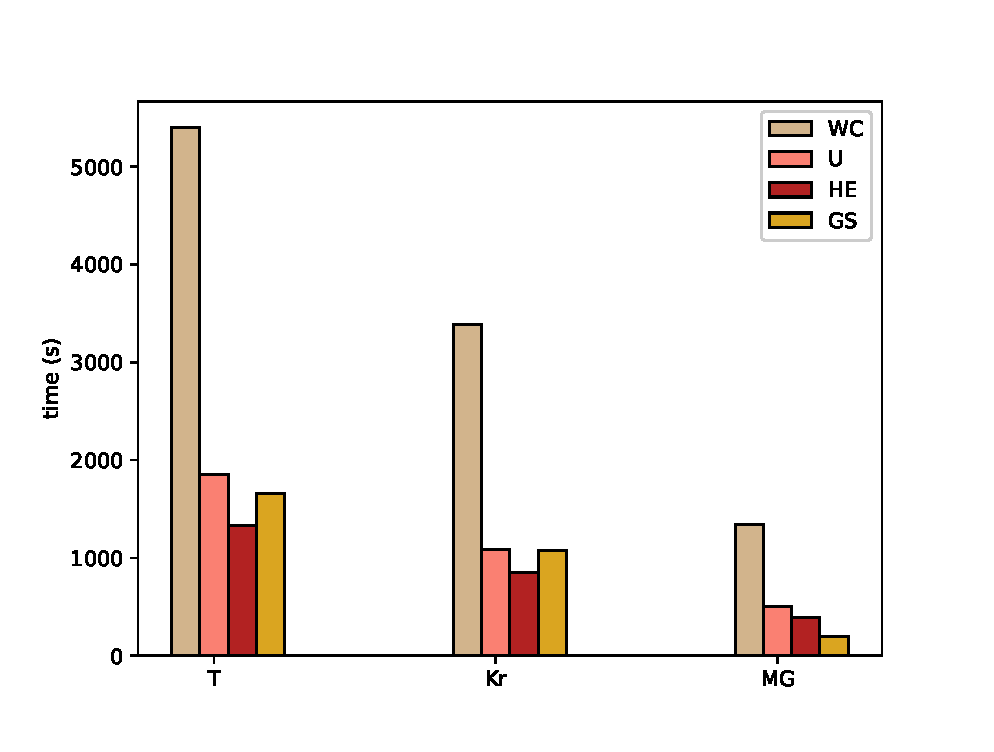
\includegraphics[width=1.0\linewidth]{figs/mg-improvement.eps}
\caption{\label{fig:mg}Wall-clock time for model components of
  Baroclinic Wave test. ``T'' denotes trunk at 17483, ``Kr'' denotes
  CSAR branch with the Krylov subspace solver and ``Mg'' denotes
  CSAR branch with the multigrid pre-conditioner as the solver.}
\end{figure} 

Displayed in Table~\ref{tab:MG_data} and shown in figure~\ref{fig:mg}
are the profiling data from CrayPAT for three different model versions
of the Baroclinic wave test on a $C1152$ mesh with a $120$s time-step
for $100$ time-steps. This corresponds to a roughly 9km
resolution. The models were run on $384$ nodes with $6$ MPI ranks per
node and $6$ Open MP threads per MPI rank.  The CSAR branch is \verb+r17264_CSAR19_gungho@17480+.

\section{PSyclone optimisation for annexed dofs}

The parallel code generated by the PSyclone tool can be modified by
PSyclone configuration options and by bespoke transformation scripts
that can apply to parts of the code or the whole code. This section
describes a change to the code generated by PSyclone and the benefits
it delivered.

The LFRic data model has a concept of ``annexed dofs''. Annexed dofs
relate to data points that are shared between cells owned by two or
more different distributed memory partitions. This is illustrated in
Figure~\ref{fig:dofownership} which shows four partitions {\tt P0} to
{\tt P3} and in particular the halos and dofs for Partition 1. In this
image, the ``Owned dof'' shared by owned cells 3 and 7 in Partition 1
also exists as a dof in the cells 2 and 6 owned by Partition 0.

When a halo swap is done, the infrastructure needs to have defined
which partition holds the correct value for such shared
dofs. Assignment of ownership of these shared dofs is done as part of
the mesh partitioning algorithm at the start of the run. Where a
partition has shared dofs which it does not own, the dofs are referred
to as annexed dofs

Somewhat arbitrarily, ownership of shared dofs is assign to the
partition with the highest number which leads, in the example figure
to Partition 1 owning the dof that it shares with Partition 0. On the
other hand, the dof marked ``Annexed dof'', which is shared with all
four partitions, is owned by Partition 3 and is therefore an annexed
dof in all other partitions including Partition 1.

\begin{figure}[ht!]
\begin{center}
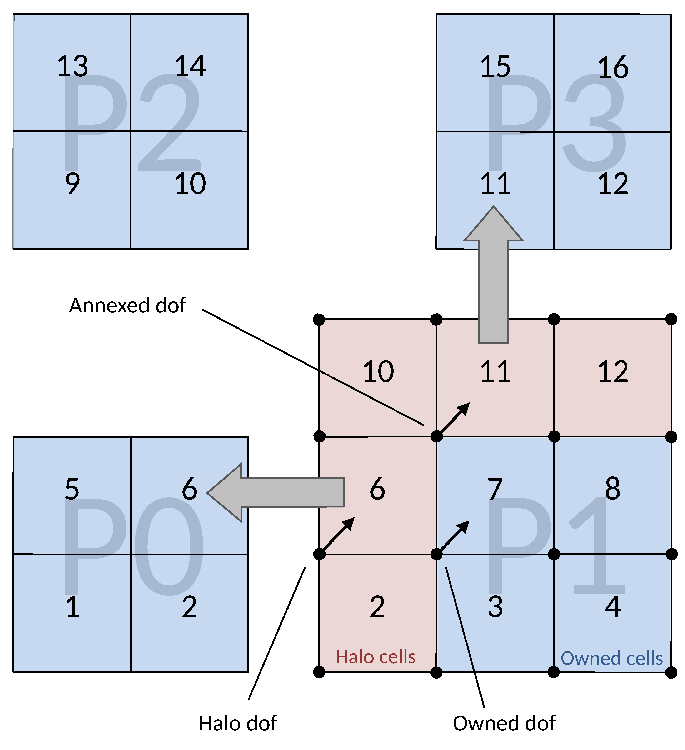
\includegraphics[scale=0.6]{figs/DofOwnership.eps}
\caption{Illustration of owned and annexed dofs. When a halo swap
  occurs Partition 0 will receive the value of the owned dof in
  Partition 1 and the annexed dof in Partition 1 will receive the
  value of the matching dof in Partition 3.}
\label{fig:dofownership}
\end{center}
\end{figure}

While science kernels are computed by looping over cells, PSyclone
supports a number of ``built-in'' operations that are computed by
looping over dofs. Such operations include initialisation of fields
and basic arithmetic operations such as adding fields or multiplying
fields by scalar values. Originally, the strategy applied by PSyclone
was to compute only the owned dofs and not the annexed dofs. The
assumption was that a halo swap would always be needed before a
built-in result would be used, and therefore computing the annexed
dofs was unnecessary.

Later it was recognised that there were operations which would not
require halo values of fields, and therefore the option was made to
compute the annexed dofs and to remove unnecessary calls to halo swap
routines.

The impact of this change was assessed and the description of the
experiment and results follows.

\subsection{Method}

The version of the trunk used in these tests was 17655 but with the same science configuration as
used in~\ref{sec:scale},
%The version of the trunk and GungHo C576 GungHo configuration that was
%assessed in \ref{sec:scale} was used for these tests, 
running on
the Cray XCS using the LFRic environment built for the Intel compiler
version 17.0.0.098. Configurations were run on 24, 54 and 96 nodes
with 6 OpenMP threads per rank. 

The difference between the control and test runs was a PSyclone
configuration setting that, by default, modified the loop limits for
all built-ins to loop either over owned dofs or over annexed dofs.
Additionally, following some initial trials and analysis, the standard
optimisation script within GungHo was modified to override this
default for those built-ins which initialise new fields: {\tt
  setval\_c} and {\tt setval\_x} which respectively initialise a field
to a constant value, and set the value of one field to another. This
additional change prevents uninitialised halo data being accessed when
a newly initialised continuous field is passed into a kernel which
increments its value. The setting will become the default for a future
version of PSyclone.

\subsection{Results and analysis}

The questions to be answered are: what impact does this change have on
the number of halo swaps required and what is the cost in time saved
from reduced halo swaps relative to the increase in time for the extra
calculations.

For an example field in the 96-node job, the number of owned and
annexed dofs was 318,096. The number of annexed dofs varies from
partition to partition, but the maximum number was 7200. This equates
to 2.2 percent additional redundant computation for annexed dof
operations which likely comprise a minority of the total cost of
computation. As the PSyclone-generated loops that implement the
built-in operations are scattered through the PSy layer code it is not
currently possible to add instrumentation to measure their cost.

LFRic infrastructure enables the number of halo swaps to be
counted. For the two scenarios, the number of halo swaps was reduced
by 52\% from 9120 per time-step for the control job to 4360 per
time-step.  Table~\ref{tab:annex} lists the cost of the halo swaps in
each of the tasks recorded by Cray PAT as the cost of the
\verb+xt_exchanger_mix_isend_irecv_s_exchange+. As can be seen, the
savings should comfortably outweigh the cost of the redundant
computation.


\begin{table}[ht!]
\scriptsize
  \begin{center}
    \caption{Percentage cost of halo swap}
    \label{tab:annex}
     \begin{tabular}{|c|c|c|}
      \textbf{Nodes} & \textbf{Original} & \textbf{Annexed dofs} \\
      \hline
      24 & 5.3  & trace  \\ 
      54 & 8.7  & 3.4    \\ 
      96 & 10.7 & 4.8    \\ 
      216 & 12.0 & -    \\ 
      384 & 13.0 & -    \\ 
    \end{tabular}
  \end{center}
\end{table}

Note that the cost of a single halo swap rises with the increase in
node count, and while the annexed dof version was not re-run on larger
node counts, the figures from the control run are listed in the table
to give an idea of the likely benefit. 







\section{I/O}
The majority of the I/O infrastructure delivering diagnostic output in the form of UGRID-NetCDF via XIOS is on the LFRic trunk
and will be used as part of the Aquaplanet runs in 2019. Therefore it is now necessary to begin regular monitoring of the impact
of I/O on compute performance. In 2017, following the preliminary integration of XIOS into the LFRic infrastructure, performance
tests were done, focussing mainly on strong scaling of LFRic-XIOS for diagnostic output. The conclusion was that XIOS scaled well
out to 384 nodes (approx. 14K cores). A description of the work plus full results can be found in \cite{Adams2018}. 

For the 2019 report, the focus is on two main areas: strong scaling when outputting regular
diagnostics and also tests of in-situ post-processing. In particular tests have been done of time-meaning and also regridding 
from the LFRic native cubed-sphere mesh to a regular lat-lon mesh. Both of these are use cases from the upcoming Aquaplanet
runs and also evaluation of XIOS regridding is of interest to the wider Next Generation Modelling Systems programme as it
could inform how downstream processing will be handled. For instance whether LFRic can deliver Level 1 data directly to StaGE.
It could also make verification of LFRic easier if the data can be directly produced on a lat-lon mesh. The aim of the post-processing
experiments described here is primarily to get an idea of computational overhead in terms of runtime and memory, 
so there is no in depth analysis of scientific accuracy apart from verifying that the jobs have produced the right kind of output. 

\subsection{Job Setup}
All tests were performed on XCS. The executables were built from LFRic at r17102 using the LFRic Intel Fortran environment (17.0.0.098) 
including the latest PSyclone 1.7.0 and XIOS at r1537 of the XIOS trunk. Build flags were the default fast-debug which equates to:
-g -traceback -warn all -warn errors -ftrapuv -check all -fpe0 -O0 -stand f08

The science configuration was the standard baroclinic wave test with timestep length dependent on mesh resolution. 
For the purposes of the tests here: 900s for a C96 mesh and 180s for a C576 mesh.
10 fields are currently output as diagnostics in this configuration (air\_density (rho), three components of vorticity (xi1, xi2, xi3), eastward\_wind (u1), 
northward\_wind (u2), exner pressure (exner), divergence
of wind (divergence) on 30 half levels; air\_potential\_temperature (theta), upward\_air\_velocity (u3) on 31 full levels
which results in approximately 5 GB data per output

To keep within the PBS queue time limit the basic run is for 120 timesteps, with diagnostic\_frequency set to 20 timesteps.
This makes for 6 writes to a single UGRID-NetCDF file over the course of the run.

\subsection{Glossary of terms}

 
\begin{itemize}
  \item Client Ratio (CR).The percentage of time a client (model) task waits for the server. Ideally it should be as close to zero as possible.
  \item Client I/O time. The actual time (seconds) that the client task spends in I/O related activity
\end{itemize} 



\subsection{Set 1: Strong scaling}

This set of tests used a C576 mesh (approx 17Km horizontal resolution). Pure MPI only (\$OMP\_NUM\_THREADS=1). 
I/O setup used 12 XIOS servers with lustre stripe set count to be the same. This was the best performing setup from
the last set of I/O performance tests, so the assumption is that it is a good starting point.

\begin{table}[ht!]
\scriptsize
  \begin{center}
    \caption{Strong Scaling: Runtime}
    \label{tab:table1}
     \begin{tabular}{|c|c|c|c|c|c|}
      \textbf{Nodes} & \textbf{Max CR~(\%)} & \textbf{Max Client IO~(s)} & \textbf{Runtime no IO~(s)} & \textbf{Runtime~(s)} & \textbf{\% incr IO}\\
      \hline
      24 & 0.002 & 12.76 & 9832 & 10115 & +3\\
      54 & 0.002 & 13.30 & 4709 & 4950 & +5\\
      96 & 0.006 & 13.36 & 2810 & 2795 & -0.5\\
      216 & - & - & - & - & - \\
      384 & - & - & - & - & - \\
    \end{tabular}
  \end{center}
\end{table}

\begin{table}[ht!]
\scriptsize
  \begin{center}
    \caption{Strong Scaling: Memory Usage *}
    \label{tab:table2}
     \begin{tabular}{|c|c|c|c|}
      \textbf{Nodes} & \textbf{Memory Usage Gb (No IO)} & \textbf{Memory Usage Gb} & \textbf{\% incr IO} \\
      \hline
      24 & 764.3 & 841.3 & +10 \\
      54 & 936.8 & 1020.2 & +8 \\
      96 & 1126.4 & ? & ? \\
      216 & - & - & -  \\
      384 & -  & -  & -  \\
    \end{tabular}
  \end{center}
\end{table}

\scriptsize \textbf{* Note some job output does not include the PBS epilogue and so memory usage is not available (indicated by ?)}
\newline

\normalsize
The results are very similar to those done in the 2016/2017 tests (which were done with a C288 mesh). For the 24, 54 and 96 node jobs we see
evidence that scaling is preserved from the decreasing run times. The Client Ratio (CR) is very close to zero in all cases, 
showing that model client tasks are hardly waiting at all for I/O requests to be processed and that I/O is asynchronous.
The \% runtime penalty for I/O is low and well within the assumed machine variability. The \% memory usage penalty for I/O is approx 8-10\%. 

216 and 384 node jobs crashed out within the first few timesteps with XIOS-related errors even though no I/O was
actually happening at those timesteps. We assume that further tuning is needed for these higher node-count jobs.
See the Conclusions section for suggested avenues to explore.

\subsection{Set 2: In-situ Post-processing}

In this set of tests the focus is on regridding and simple time-meaning, with usage examples taken from latest Aquaplanet branch.
The aim here is to get an idea of computational overhead in terms of runtime and memory, and general correctness rather than scaling.
Therefore, these tests were done with a lower-resolution C96 mesh and only out to 96 nodes.
Runs have also been done to compare run time and memory usage to the same job configuration with only regular diagnostic output and also 
no I/O to get an idea of the additional penalty for using XIOS post-processing. 

\subsubsection{Averaging}

As Set 1, with the following changes: C96 mesh, 900s timestep.
In addition to regular diagnostics, averages are output over 20 timesteps, giving 6 writes to an additional file. 

\normalsize
\begin{figure}[ht!]
  \begin{center}
   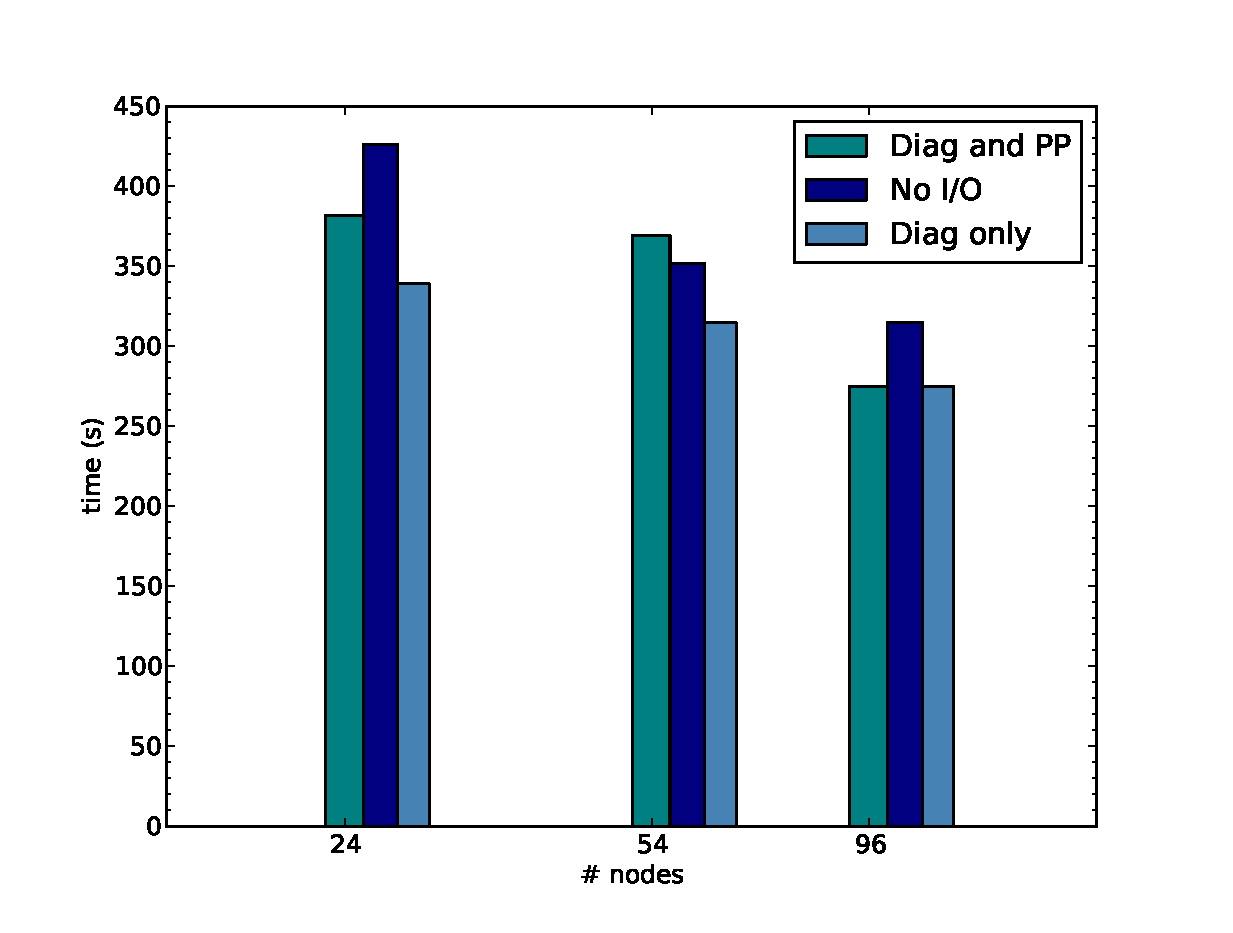
\includegraphics[scale=0.4]{figs/ave.eps}
   \caption{Averaging}
   \label{fig:fig1}
  \end{center}
\end{figure}

\begin{table}[ht!]
\scriptsize
  \begin{center}
    \caption{Averaging: Runtime}
    \label{tab:table3}
     \begin{tabular}{|c|c|c|c|c|c|}
      \textbf{Nodes} & \textbf{Max CR~(\%)} & \textbf{Max Client IO~(s)} & \textbf{Runtime~(s)} & \textbf{\% incr diag IO} & \textbf{\% incr no IO}\\
      \hline
      24 & 0.02 & 1.63 & 382 & -11 & +11 \\ 
      54 & 0.03 & 0.90 & 369 & +5 & +19 \\ 
      96 & 0.04 & 2.90 & 275 & -14 & 0 \\ 
    \end{tabular}
  \end{center}
\end{table}

\begin{table}[ht!]
\scriptsize
  \begin{center}
    \caption{Averaging: Memory Usage}
    \label{tab:table4}
     \begin{tabular}{|c|c|c|c|}
      \textbf{Nodes} & \textbf{Memory Usage Gb (pp) } & \textbf{Memory Usage Gb (diag only)} & \textbf{Memory Usage Gb (no IO)} \\
      \hline
      24 & 82.9 & 81.8 & 77.4 \\
      54 & 150.9 & 149.2 & 138.8 \\
      96 & 234.1 & ? & ? \\
    \end{tabular}
  \end{center}
\end{table}


Figure \ref{fig:fig1} gives a quick overview of scaling comparing run times for jobs without I/O, with regular diagnostic output and with
regular diagnostic output plus averaging. Scaling is still evident as run times generally decrease with the number of nodes. From
Table \ref{tab:table3}, the \% increases over just diagnostic output and no I/O are inconclusive - sometimes positive and sometimes negative. 
The range seems to be greater than for Set 1 so maybe a 5-10\% runtime penalty can be inferred, but it is difficult to say 
without doing runs to assess run time variability. Table \ref{tab:table4} shows a clear memory usage increase when adding different types of I/O. 
About +6-7\% for diagnostic I/O over runs with no I/O and a further +1\% for adding averaging post-processing. 


\subsubsection{Regridding}

As Set 1, with the following changes: C96 mesh, 900s timestep.
In addition to regular diagnostics, the rho, exner and divergence fields are regridded (to N96 equivalent) and output every 20 time steps, giving 6 writes to an additional file. Two sets of runs were done: computing weights on-the-fly each time and also using precomputed weights.

\normalsize
\begin{figure}[ht!]
  \begin{center}
   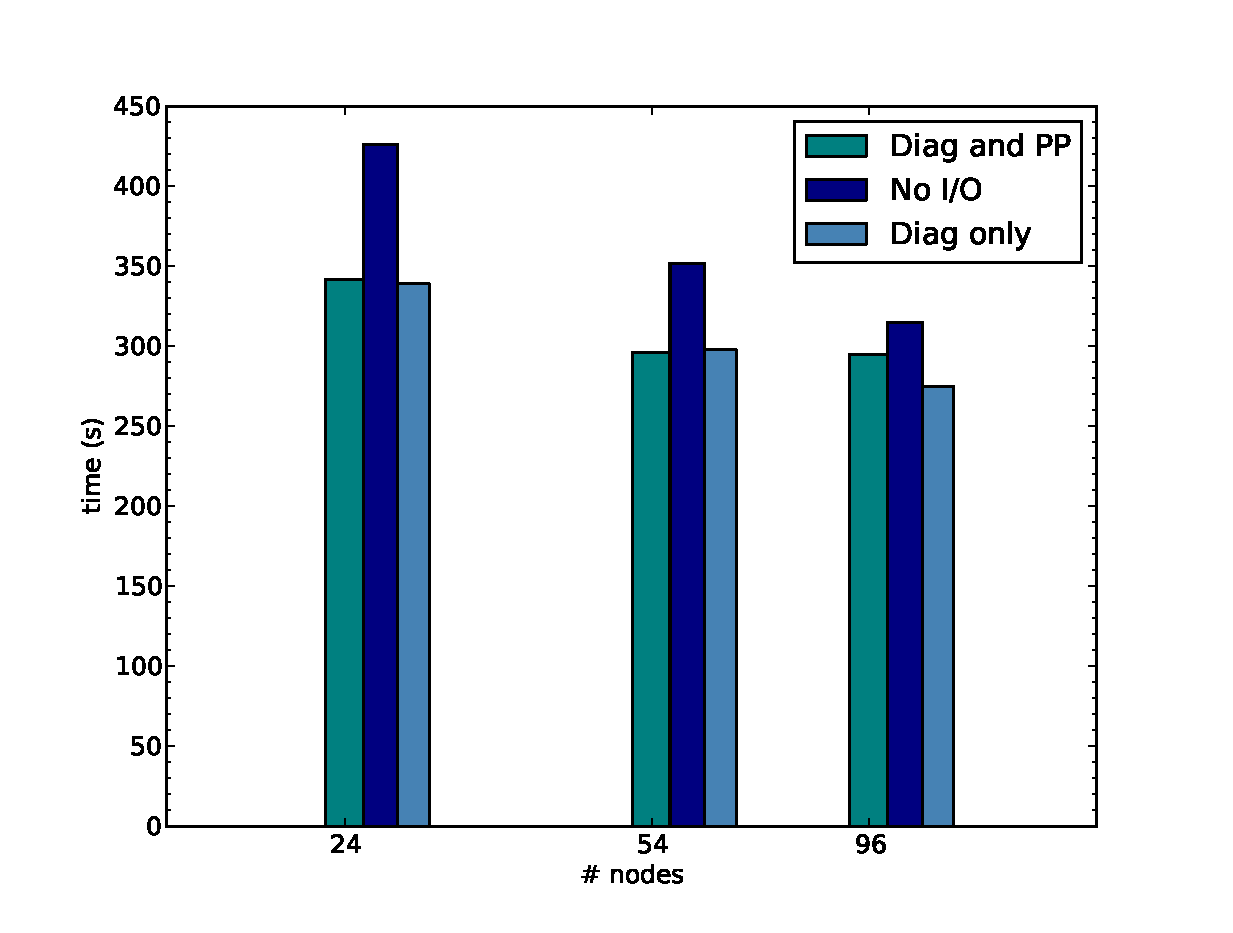
\includegraphics[scale=0.4]{figs/regrid.eps}
   \caption{Regridding (computing weights)}
   \label{fig:fig2}
  \end{center}
\end{figure}

\begin{figure}[ht!]
  \begin{center}
   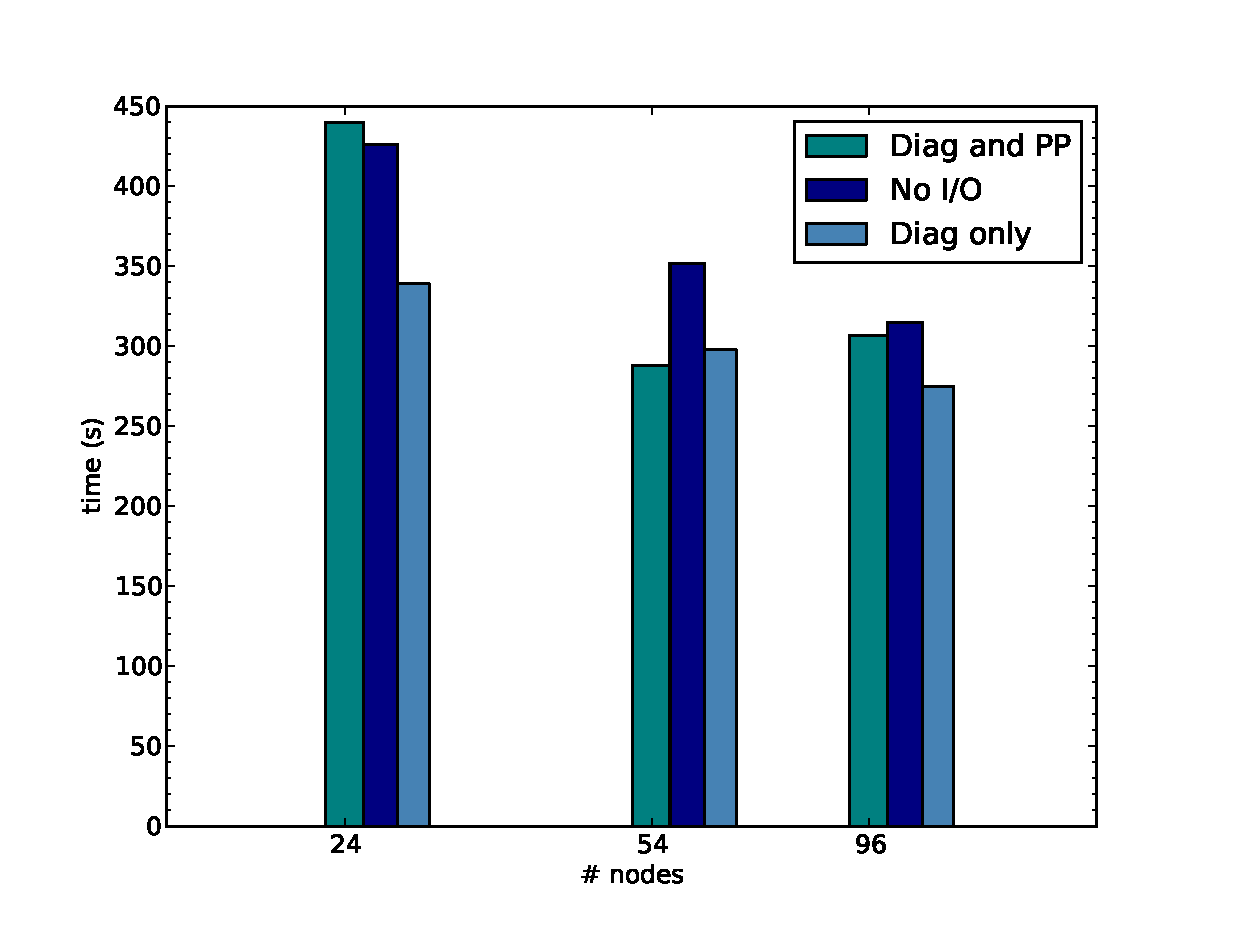
\includegraphics[scale=0.4]{figs/regrid_pcw.eps}
   \caption{Regridding (precomputed weights)}
   \label{fig:fig3}
  \end{center}
\end{figure}

\begin{table}[ht!]
\scriptsize
  \begin{center}
    \caption{Regrid, computing weights: Runtime}
    \label{tab:table5}
     \begin{tabular}{|c|c|c|c|c|c|}
      \textbf{Nodes} & \textbf{Max CR~(\%)} & \textbf{Max Client IO~(s)} & \textbf{Runtime~(s)} & \textbf{\% incr diag IO} & \textbf{\% incr no IO}\\
      \hline
      24 & 0.03 & 9.10 & 342 & -24 & +0.9 \\ 
      54 & 0.04 & 9.89 & 296 & -19 & -0.6 \\
      96 & 0.05 & 17.01 & 295 & -7 & +7 \\
    \end{tabular}
  \end{center}
\end{table}

\begin{table}[ht!]
\scriptsize
  \begin{center}
    \caption{Regrid, computing weights: Memory Usage}
    \label{tab:table6}
     \begin{tabular}{|c|c|c|c|}
      \textbf{Nodes} & \textbf{Memory Usage GB (pp) } & \textbf{Memory Usage GB (diag only)} & \textbf{Memory Usage GB (no IO)} \\
      \hline
      24 & 83.0 & 81.8 & 77.4 \\
      54 & 150.6 & 149.2 & 138.8 \\
      96 & ? & ? & ? \\
    \end{tabular}
  \end{center}
\end{table}

\begin{table}[ht!]
\scriptsize
  \begin{center}
    \caption{Regrid, precomputed weights: Runtime}
    \label{tab:table7}
     \begin{tabular}{|c|c|c|c|c|c|}
      \textbf{Nodes} & \textbf{Max CR~(\%)} & \textbf{Max Client IO~(s)} & \textbf{Runtime~(s)} & \textbf{\% incr diag IO} & \textbf{\% incr no IO}\\
      \hline
      24 & 0.02 & 7.07 & 440 & +3 & +30 \\
      54 & 0.04 & 3.30 & 288 & -18 & -3 \\
      96 & 0.04 & 4.32 & 307 & -3 & +12 \\
    \end{tabular}
  \end{center}
\end{table}

\begin{table}[ht!]
\scriptsize
  \begin{center}
    \caption{Regrid, precomputed weights: Memory Usage}
    \label{tab:table8}
     \begin{tabular}{|c|c|c|c|}
      \textbf{Nodes} & \textbf{Memory Usage Gb (pp) } & \textbf{Memory Usage Gb (diag only)} & \textbf{Memory Usage Gb (no IO)} \\
      \hline
      24 & 85.4 & 81.8 & 77.4 \\
      54 & 153.0 & 149.2 & 138.8 \\
      96 & 248.2 & ? & ? \\
    \end{tabular}
  \end{center}
\end{table}

\normalsize

From looking at the comparative runtimes in Figures \ref{fig:fig2} and \ref{fig:fig3} alone there is no clear benefit of computing weights each time vs using precomputed weights. As in previous results the general run time variability obscures things. Scaling is still evident as run times generally decrease with
increasing node count. Table \ref{tab:table7} gives a slight hint that client performance improves when using precomputed weights (lower CR and time spent in I/O).
Interestingly, memory usage increases slightly. Presumably there is a trade-off between the time and resources spent reading in the weights vs computing them.

\subsection{Conclusions}

Compared to the previous I/O performance assessment, in this year's tests the mesh resolution has been doubled and many more fields are output (although fewer timesteps are being run). A first assessment of the cost of in-situ post-processing has been made and is generally encouraging in that it seems to work correctly and there is no severe overhead of adding post-processing on top of regular diagnostic output. However, to get a really clear picture a thorough analysis of runtime variability for all non-I/O, diagnostic and post-processing scenarios is necessary. The post-processing tests need to be repeated with a higher resolution mesh as it may make any penalty more obvious (e.g. when computing regridding weights on the fly vs using precomputed weights). The issues seen with higher node count jobs need addressing to find out the cause. In the last I/O performance assessment no such problems were seen with 216 and 384 node jobs but many things have changed since then: the mesh is higher resolution and the LFRic dynamics and physics science schemes have changed considerably. 
We suggest several avenues of investigation:

\begin{itemize}
  \item XIOS buffer size. Normally not recommended to change this, but worth looking at as the error messages were to do with buffering and message passing
  \item Trying many more I/O servers
  \item Partial occupancy of nodes. If this is a memory problem then not fully occupying the nodes may help.
  \item Memory usage investigations to look at how memory usage changes during the run and what happens prior to a crash.
\end{itemize}


It is suspected that the issues are to do with memory usage and to
fully investigate this LFRic needs a way of regularly monitoring
per time-step memory usage as a matter of urgency.
 



\section{Optimisation for Processor Architectures
\label{sec:pa}}

\subsection{NVIDIA GPU}
The LFRic-microbenchmark suite~\cite{lfric-microbenchmarks} allows
optimisations for individual kernels to be explored without having to
compile and run the whole code. This is particularly useful when
targeting a programming model such as OpenACC for GPU architecture
where the Portland group compiler cannot compile the Fortran 2003 used 
in the main code.

The local matrix assembly (LMA) matrix-vector kernel had been
previously ported to run on GPUs by inserting Open ACC directives in
the PSy layer code to control the data transfer from host memory to
device memory and to offload the kernel call to the GPU device. This
Open ACC version was the starting point for Alan Gray from NVIDIA to
to look at optimisations. Moreover, after discussions regarding 
the PSyKAl API and the LFRic plans for how Open ACC will be
implemented for a GPU version, NVIDIA believe that the plan and
implementation will enable a succesful GPU implementation.
This is a summary of potential optimisations from NVIDIA.

\begin{lstlisting}[language=Fortran,caption={Code fragment of original 
    kernel},label={lst:LMA-orig}]
  !$acc loop vector 
  do k = 0, nlayers-1
    lhs_e(:,:) = 0.0_r_def
    ik = (cell-1)*nlayers + k + 1

    do df = 1, ndf1
      do df2 = 1, ndf2
        lhs_e(df,k) = lhs_e(df,k) + & 
          matrix(df,df2,ik)*x(map2(df2)+k)
      end do
    end do

    do df = 1, ndf1
      lhs(map1(df)+k) = lhs(map1(df)+k) + lhs_e(df,k)
    end do

  end do 
  !$
\end{lstlisting}

Shown in listing~\ref{lst:LMA-orig} is a code fragment of the LMA
kernel. It has an Open ACC directive \verb+!$acc loop vector+ before the
outmost $k$ loop, so that each thread in a thread block will do different loop
iterations. This code runs on a GPU, but not very efficiently. 

The first optimisation was to fuse the two loops over \verb+ndf1+
(lines 6-11 and 13-15) and replace the array \verb+lhs_e+ with a
scalar. The scalar can stay resident in a register for each thread and
avoids unnecessary memory accesses. This optimisation is call loop
fuse. 

The second optimisation was to exploit more parallelism on the GPU.
This performed with the Open ACC loop clause {\em collapse} to combine
the two outermost loops. This has the added benefit of aiding {\em
  memory coalescence}, {\em i.e.} neighbouring parallel threads
accessing neighbouring memory locations. However, an Open ACC {\em
  atomic update} directive is required as the loop over {\em ndf1} is
now also parallel. This optimisation is called Loop collapse. The new
kernel code is shown in listing~\ref{lst:LMA-opt}. 

\begin{lstlisting}[language=Fortran,caption={Optimised
    kernel},label={lst:LMA-opt}]
  !$acc loop vector collapse(2)
  do k = 0, nlayers-1
    do df = 1, ndf1

      ik = (cell-1)*nlayers + k + 1
      lhs_e_scal = 0.0_r_def

      do df2 = 1, ndf2
         lhs_e_scal = lhs_e_scal + & 
            matrix(df,df2,ik)*x(map2(df2)+k)
      end do
      
      !$acc atomic update
      lhs(map1(df)+k) = lhs(map1(df)+k) + lhs_e_scal

    end do
  end do
\end{lstlisting}

These first two optimisations increase the speed of execution but the
code still has a large register usage which results in low occupancy
of the GPU parallel units. This can be reduced by inlining the kernel
subroutine into the PSy layer. This can be done by the PGI compiler,
using Inter-procedural Analysis (IPA). This triggered by the following
compiler flag \verb+-Mipa=inline:reshape -Minfo flags+. The info flag
is for reporting purposes. This optimisation is called Inlining. 

The final optimisation is to note that the kernel is launched multiple
times, as the PSy layer includes the colouring ordering code for serialisation
to prevent race conditions. The kernel executes faster with a
single launch and NVIDIA optimised this by loop collapsing the loop
over colours and cells per colour. In the full code, this could be
simply done by not colouring at all. This optimisation is called
Single Kernel.

The colouring serialisation loop order is done for correctness,
however, the presence of the atomic update in the kernel prevents the
data race that colouring is designed to prevent, so the code is thread
safe. However, the atomic update doesn't guarantee the order of
execution, whereas colouring does. This means that whilst the data
race is avoided with the atomic update, the answer is not reproducible against
multiple runs. This is an optimisation which could be chosen for speed
when reproducibility is not an issue.

Shown in Table~\ref{tab:lma_nvidia} are the execution times for each
optimisation and in figure~\ref{fig:lma_nvidia} is shown the resulting
speed up versus the original code version.

\begin{table}
\centering
\caption{\label{tab:lma_nvidia} Execution times for different
  optimisations of a single run of  the LMA kernel on an V100 
  {\em Volta} NVIDIA GPU.}
\begin{tabular}{rc}
Optimisation & time (ms) \\\hline
Original     & $9.45$ \\
Loop fusion  & $5.33$ \\
Loop collapse & $2.68$ \\ 
Inlining      & $0.58$ \\
Single Kernel & $0.32$ \\\hline
\end{tabular}
\end{table}

\begin{figure}
\centering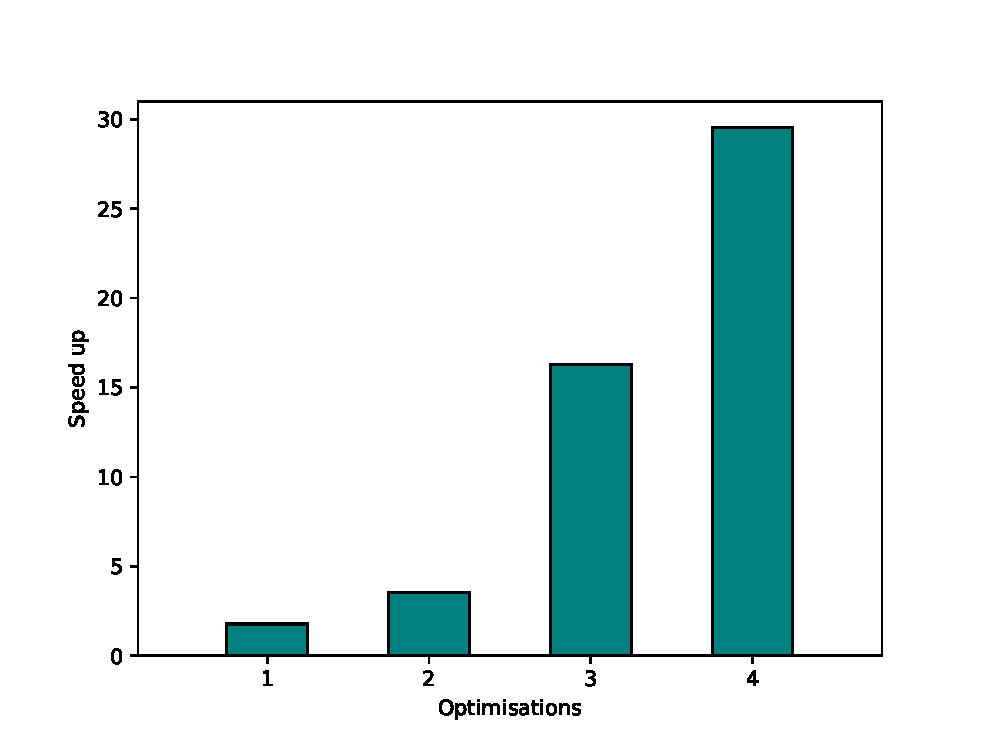
\includegraphics[width=1.0\linewidth]{figs/LMA-nvidia.eps}
\caption{\label{fig:lma_nvidia}Speed up of the LMA kernel against the
  original code for various optimisations. 1 loop fusion. 2 loop
  collapse. 3 Inlining. 4 Single Kernel.}
\end{figure} 

The speed up times are impressive, but a further analysis of the
absolute performance is useful. The NVIDIA profiler was
used to measure some performance metrics. This was compared to a simple ``roofline''
analysis~\cite{roofline} of the code on Volta. This suggests that as the arithmetic
intensity (flops per byte) of $0.3$ flops/byte of the kernel is low
compared to the ridge-line of the hardware, $9.9$ flops/byte, then the
code is memory bound. Comparing the memory bandwidth achieved of 549
GB/s to the Stream benchmark for the hardware suggests the code is
achieved around $70\%$ of the available bandwidth. This suggest the
code is fairly well optimised.

It should be noted that the problem size is too small, the data file
supplied to NVIDIA had $864$ cells with $40$ layers. Whilst, a target
local volume size of $12\times 12=144$ or $24\times 24=576$ is a
reasonable size for a single core of a CPU, a similar size is too
small to fully exploit the parallelism of GPU. In particular, to
effectively exploit the SIMT parallelism with the vertical degrees of
freedom, the vector size should be $128$ or more. $40$ levels is
clearly to few. Worse, in this particular case the colouring data here
had the non-optimal $6$ colours, whereas $4$ is sufficient. As seen in
the previous year's performance report the GPU should handle much more
work for a disproportional decrease in cost. This is especially true
for the number of levels.

These optimisations show that the code can run with some degree of
efficiency on a GPU. PSyclone is being developed so that is can
produce the necessary Open ACC directives in the PSy layer. Moreover,
its is being developed so that it can parse individual statements in
the kernel. This is necessary so that the kernel source can be
annotated with directives. Then the whole code can have a GPU
implementation generated automatically. To modify the actual source
code takes this a step further. However, it would in principle be
possible and moreover, this is similar to some of the ideas in CLAW~\cite{claw}.
CLAW is being considered for the parallelisation of the physical
parameterisations and some of the ideas would then be re-implemented in
PSyclone. Generating optimised code for GPUs is then possible.



\section{CMA micro-benchmark on Broadwell and TX2}
In this section we will introduce the CMA\_appinv micro-benchmark and present performance results from tests on the Intel Broadwell and Cavium ARM-based ThunderX2 architectures.
In addition we compare performance of the micro-benchmark when built with different compilers and runtime libraries.

\subsection{CMA micro-benchmark}

The LFRic dynamical model performs operations to solve
\begin{equation} \label{eq:matvec}
A \cdot \mathbf{x} = \mathbf{b}
\end{equation}
in various guises and contexts where $A$ is a matrix representing a partial differential equation, $\mathbf{b}$ is a vector containing information describing boundary conditions and $\mathbf{x}$ is a state vector.
The finite element methods that the GungHo application uses are written to perform operations on a cell-by-cell basis in what is termed Local Matrix Assembly (LMA).
The LMA micro-benchmark discussed in the previous report is a characteristic example of such methods.
The LFRic infrastructure also contains methods for solving equation \ref{eq:matvec} on a column-by-column basis.
Although these Column Matrix Assembly (CMA) methods have yet to be utilised by the full GungHo application they are deployed in the gravity\_wave mini-app.

For this report we generated a new CMA micro-benchmark using LFRic revision 15378 focused on the columnwise\_op\_appinv\_kernel\_code() routine in the gravity\_wave mini-app.
This kernel is used in the pre-conditioner for the Helmholtz solver.
As per the LMA micro-benchmark described in the previous report, the driver code was extracted from the Psyclone-generated Psy-layer and the kernel was taken directly from the LFRic source code.
By design, the driver routine contains the so called global optimisations, namely OpenMP worksharing and colouring (to prevent race conditions) over columns on the sphere.

The dinodump capability from PYSKE was used to generate Known Good Output (KGO) which we use to verify the micro-benchmark behaved as expected in later tests.
This involved adding additional PSYKE subroutine calls to the Psy-layer code in the gravity\_wave mini-app in order to capture the input scalars and arrays for the kernel.
The micro-benchmark driver code was also trivially modified to read in the produced dinodump before calling the kernel and compare the result of the kernel against the KGO.
Before running the mini-app to generate the dinodumo the number of vertical layers in the configuration was modified from the default (10) to 256.
While current NWP and climate GA and RA production configurations use between 70 and 90 vertical (UM) levels we took 256 layers in order to increase the throughput of the benchmark and also in expectation that future configurations will run with increased vertical resolution.


While generating the new micro-benchmark a minor bug in kernel was discovered.
Specifically, the manner in which the kernel is called in gravity\_wave mini-app (and the supporting code comments) indicate that the kernel is called to update the target array but instead the kernel actually populates the array while overriding the initial contents.
It was confirmed by the original author of the code that the functionality of the kernel was correct and the comments are in error.
The bug has minimal performance impact on CPU architectures- an intent(inout) array should be intent(out)- but may have a larger impact on GPU architectures where the array would be being offloaded unnecessarily. 

The resultant micro-benchmark can be found in the micro-benchmark ~\cite{lfric-microbenchmarks} suite on github.
We note at this point when making comparisons between the LMA and CMA\_appinv micro-benchmarks we should be mindful that they serve different purposes in the solver code.
Specifically, the LMA micro-benchmark applies the matrix $A$ to a vector $\mathbf{x}$ whereas the CMA\_inv micro-benchmark applies the inverse matrix $A^{-1}$ to $\mathbf{b}$, in other words it solves equation \ref{eq:matvec} for $\mathbf{x}$.

\subsection{CMA\_appinv performance}

We present timings for the kernel on Intel Broadwell and Cavium ThunderX2 as measured using omp\_get\_wtime().
In each case the kernel was run for 1000 iterations in order to obtain a smooth out runtime variability.
% Timing the routine in this way may however slightly exaggerate the time spend performing thread synchronisation, a cost we estimate to be within the noise of the system.
We use the latest stable version of each compiler available on the two platforms at the time of writing.
Each executable was built with the -O3 optimisation flag.

\subsubsection{Intel Broadwell}
On the Broadwell platform used (XCS) the compilers used were
\begin{itemize}
\item CCE 8.7.7
\item Intel 17.0.0.098
\item GNU 7.3.0
\end{itemize}



During the development of this work we encountered notable differences in performance between compiler versions.
For example, a measurable performance degradation between cce 8.6.0 and the cce 8.7.x series.
The single threaded (OMP\_NUM\_THREADS=1) runtime increased from 7.4s to 10.5s when changing between the two versions.
In other words cce 8.6.0 produces a faster executable than the Intel compiler but the 8.7.7 executable is slower than the Intel generated version.
This discrepancy is outwith the observed run-to-run variability on the system and is unexplained at present.
We use the more recent (but slightly less performant) cce 8.7.7.

\subsubsection{TX2}
Isambard is a XC50 system hosted by the Met Office and funded by the GW4 alliance and EPSRC.
The heterogeneous system contains chips of various architectures including 164 Cavium ThunderX2 nodes.
At the time of writing (after the March 2019 upgrade to CLE7.0) the supported compilers on the ARM-based nodes are
\begin{itemize}
\item CCE 8.7.9
\item GNU 8.2.0
\item Allinea 19.0.1
\end{itemize}
where the Allinea compiler is built on top of LLVM and Flang.



\subsection{CMA\_appinv performance using drop-in library call}
Here we investigate whether the implementation of the Thomas algorithm as written in the kernel can be replaced with a call to a standard library- in this case LAPACK.
The potential benefits of this include a potential improvement to runtimes of current architectures.
But, more importantly calling a standard API allows us to tap into routines that have been optimised specifically for the architecture being used.
This could provide performance portability while reducing porting and maintenance costs when moving between future compute platforms.
A potential problem with this plan is that the memory layout used in the columnwise operator type objects differs from that expected by the LAPACK API.

The version of the micro-benchmark used can be found in a branch of the github repo.

Thread scaling
Thread-scales OK but runtime is poor.
Is it memory copies? No, we tried taking these out but couldn't match ``vanilla'' performance.

\subsection{Discussion}

It is worth noting that there are few opportunities for vectorisation in the current implementation.

In avoiding building the LFRic infrastructure we also avoid compiler support problems.
TX2 vs Broadwell
Single thread performance on Broadwell is comfortably better than TX2. However, when multithreading is considered then the machines are node-for-node comparable.
Use of drop-in lib
Use of LAPACK as a drop-in replacement for kernel. Not optimal at present- LAPACK is optimised for larger problems.

Worth investigating vectorised versions of the algorithm, especially in the context of GPUs.


\bibliography{refs.bib}
\bibliographystyle{unsrt}

\end{document}
